\chapter{Noise and Phase Noise}
\section{Overview}
We study oscillator phase noise from three complementary perspectives: (i) spectral model (Leeson), (ii) sensitivity model (ISF/PPV), and (iii) time-domain jitter integration. We then translate masks into RMS jitter and propose reduction techniques. Key references: \cite{leeson1966,hajimiri1998,demir2000,razavi_rf}.

\section{Leeson-Type Spectral Model}
At offset \(\Delta f\) from carrier \(f_0\), a simplified form is
\[
 \mathcal{L}(\Delta f) \approx 10\log_{10}\!\Bigg( \frac{F k T}{2 P_s}\,\frac{f_0^2}{Q^2\,\Delta f^2}\,\Big(1+\frac{f_c}{\Delta f}\Big) \Bigg)
\]
where \(F\) is the noise factor of the active core, \(P_s\) is the signal power in the tank, \(Q\) is the tank quality factor, and \(f_c\) is the flicker corner. The \(1/\Delta f^2\) thermal skirt and the \(1/\Delta f^3\) close-in region are captured by the factor \(1+f_c/\Delta f\).

\section{ISF / PPV Sensitivity View}
Let the phase sensitivity around the limit cycle be \(\Gamma(\theta)\) (ISF) or PPV in time domain. The contribution of a white noise current source with PSD \(S_i\) is
\[
 \sigma_\phi^2 \propto \frac{S_i}{I_{swing}^2} \int_0^{2\pi} \Gamma^2(\theta)\, d\theta
\]
High-\(Q\) tanks yield more sinusoidal waveforms and smaller \(\Gamma\) peaks, thus lowering phase noise. Balanced differential cores suppress even-order distortion and AM-to-PM conversion.

\section{From Phase Noise to RMS Jitter}
Given single-sideband \(\mathcal{L}(f)\) and carrier \(f_0\), the RMS jitter within \([f_1,f_2]\) is
\[
 \sigma_t \approx \frac{1}{2\pi f_0}\,\sqrt{2\int_{f_1}^{f_2} 10^{\mathcal{L}(f)/10}\, df}
\]
Close-in flicker often makes \(\sigma_t\) sensitive to \(f_1\); loop filtering in PLLs sets an effective lower bound (loop bandwidth).

\section{Supply and Substrate Coupling}
Supply ripple at frequency \(f_r\) modulates the control node or tail current and creates discrete spurs at \(f_0\pm f_r\). Transfer suppression uses local LDO/filters, high PSRR bias references, and routing/grounding symmetry. Quantify by injecting a small sinusoid on \(V_{DD}\) and measuring \(\Delta f\) and spur level.

\section{Illustrative Masks and Integration}
\begin{figure}[H]
  \centering
  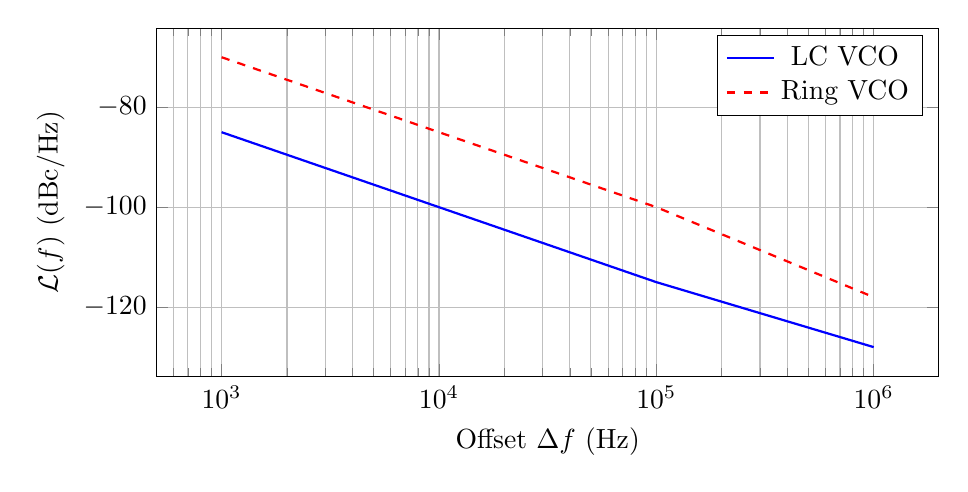
\begin{tikzpicture}
    \begin{axis}[
      width=0.95\linewidth, height=6cm,
      xmode=log, grid=both,
      xlabel={Offset $\Delta f$ (Hz)}, ylabel={$\mathcal{L}(f)$ (dBc/Hz)}]
      % LC example
      \addplot[blue, thick] table[row sep=\\]{x y \\
        1e3  -85 \\
        1e4 -100 \\
        1e5 -115 \\
        1e6 -128 \\
      };
      % Ring example
      \addplot[red, thick, dashed] table[row sep=\\]{x y \\
        1e3  -70 \\
        1e4  -85 \\
        1e5 -100 \\
        1e6 -118 \\
      };
      \legend{LC VCO, Ring VCO}
    \end{axis}
  \end{tikzpicture}
  \caption{Illustrative phase-noise masks for LC and Ring VCO}
\end{figure}

\begin{figure}[H]
  \centering
  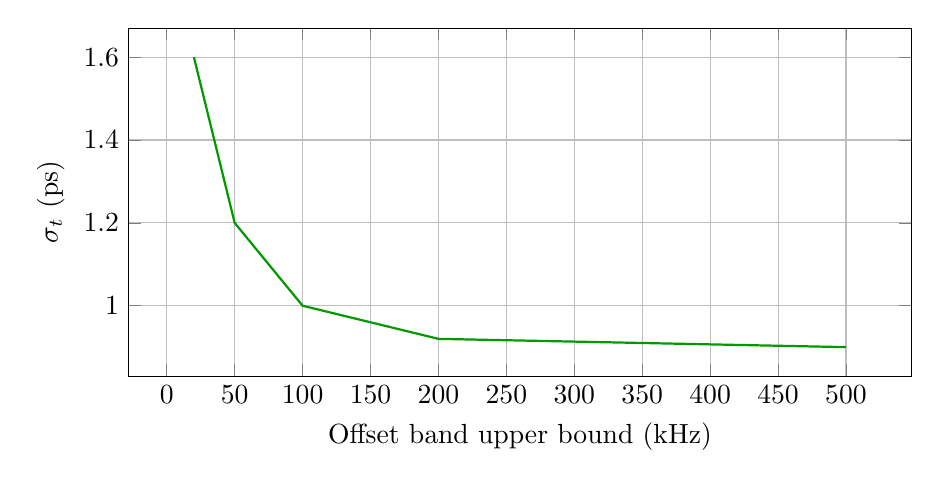
\begin{tikzpicture}
    \begin{axis}[
      width=0.95\linewidth, height=6cm,
      xlabel={Offset band upper bound (kHz)}, ylabel={$\sigma_t$ (ps)}, grid=both]
      \addplot[green!60!black, thick] table[row sep=\\]{x y \\
        20  1.6 \\
        50  1.2 \\
        100 1.0 \\
        200 0.92 \\
        500 0.90 \\
      };
    \end{axis}
  \end{tikzpicture}
  \caption{Illustrative RMS jitter vs integration band for a given mask}
\end{figure}

\section{Measurement and Simulation Flow}
\begin{itemize}
  \item PSS/Pnoise (jitter mode) over offsets from 1 kHz to 10 MHz; export \(\mathcal{L}(f)\).
  \item Transient-noise simulation to extract time-domain zero-crossing jitter; compare integrated PN to \(\sigma_t\).
  \item Bench: spectrum analyzer for far-out PN; cross-correlation PN analyzer for close-in; supply injection for PSRR and spur mapping.
\end{itemize}

\section{Reduction Techniques}
\begin{itemize}
  \item Maximize \(Q\) (inductor quality, low-loss caps), increase tank swing within reliability limits.
  \item Optimize bias for \(g_m\)/noise trade-off; filter tail current; ensure differential symmetry.
  \item Isolate supplies/grounds; use multi-band decoupling; shield high-impedance nodes.
  \item For ring VCO: increase bias to sharpen edges; multiphase averaging; consider injection locking for close-in PN.
\end{itemize}

\section{Phase-Noise Budget and Targets}
\begin{table}[H]
  \centering
  \begin{tabular}{llll}
    \toprule
    Offset band & Target $\mathcal{L}(f)$ & Dominant source & Mitigation \\
    \midrule
    1–10 kHz   & $< -80$ dBc/Hz & flicker upconversion & symmetry, bias point, AGC \\
    10–200 kHz & $< -100$ dBc/Hz & core thermal + tail & tail filtering, raise swing \\
    0.2–2 MHz  & $< -120$ dBc/Hz & tank/Q limit & higher $Q$, lower loss \\
    \bottomrule
  \end{tabular}
  \caption{Example PN budget and dominant mitigation levers}
\end{table}

\section{Inductor $Q(f)$ Illustration and Parasitics}
\begin{figure}[H]
  \centering
  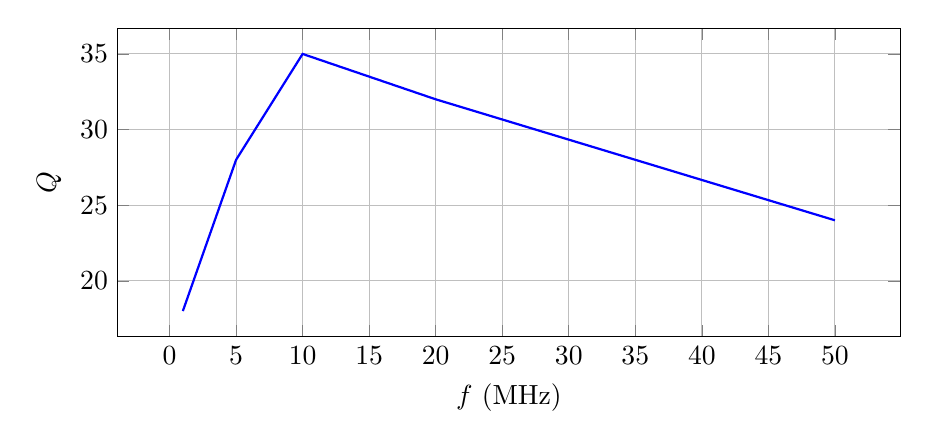
\begin{tikzpicture}
    \begin{axis}[
      width=0.95\linewidth, height=5.5cm,
      xlabel={$f$ (MHz)}, ylabel={$Q$}, grid=both]
      \addplot[blue, thick] table[row sep=\\]{x y \\
        1   18 \\
        5   28 \\
        10  35 \\
        20  32 \\
        50  24 \\
      };
    \end{axis}
  \end{tikzpicture}
  \caption{Illustrative inductor quality factor vs. frequency}
\end{figure}

\begin{table}[H]
  \centering
  \begin{tabular}{lll}
    \toprule
    Parasitic & Typical value & PN impact \\
    \midrule
    Metal series $R_s$ & 0.4–1.2 $\Omega$ & lowers $Q$, raises far-out PN \\
    Substrate $C_{sub}$ & 50–200 fF & adds loss, close-in PN via $Q$ \\
    Varactor $R_p$ & 1–5 k$\Omega$ & AM-to-PM path, 1/f folding \\
    Tail current noise & nA/$\sqrt{\text{Hz}}$ & upconverts to phase \\
    \bottomrule
  \end{tabular}
  \caption{EM/parasitic summary and qualitative phase-noise effects}
\end{table}

\section{ISF Illustration}
\begin{figure}[H]
  \centering
  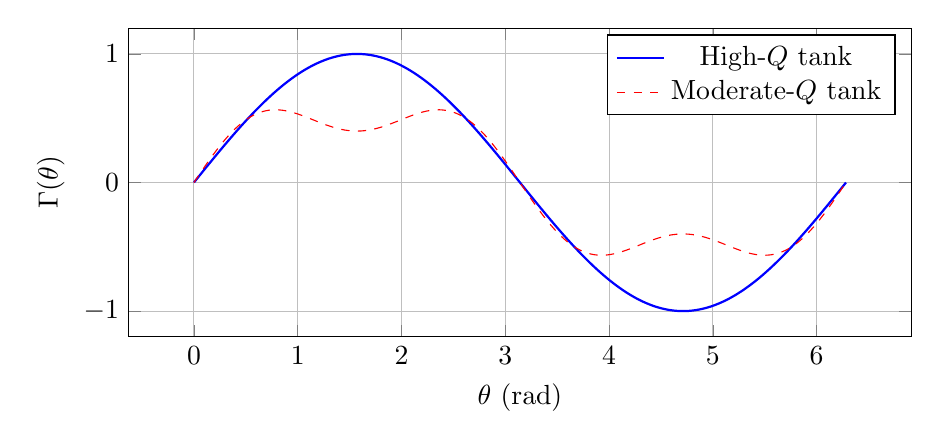
\begin{tikzpicture}
    \begin{axis}[
      width=0.95\linewidth, height=5.5cm,
      xlabel={$\theta$ (rad)}, ylabel={$\Gamma(\theta)$}, grid=both]
      \addplot[blue, thick, domain=0:6.283, samples=200] {sin(deg(x))};
      \addplot[red, dashed, domain=0:6.283, samples=200] {0.6*sin(deg(x)) + 0.2*sin(deg(3*x))};
      \legend{High-$Q$ tank, Moderate-$Q$ tank}
    \end{axis}
  \end{tikzpicture}
  \caption{Qualitative ISF: higher-$Q$ tanks yield smoother, smaller sensitivity}
\end{figure}

\section{Supply Sensitivity Map}
\begin{figure}[H]
  \centering
  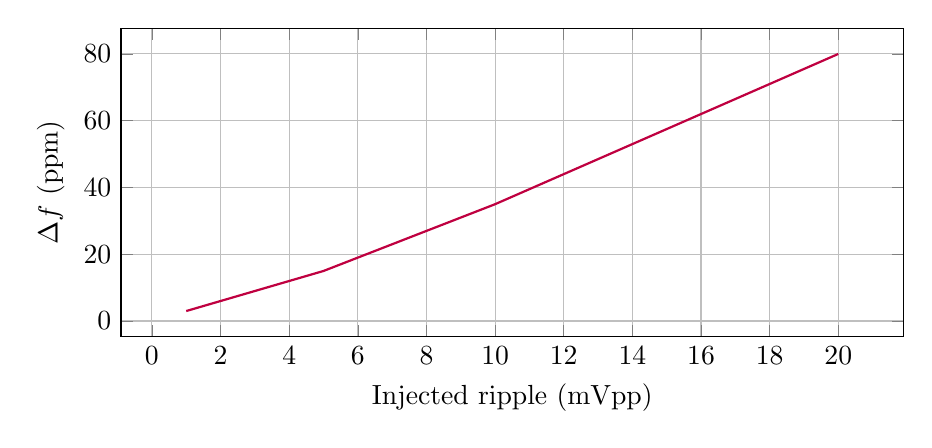
\begin{tikzpicture}
    \begin{axis}[
      width=0.95\linewidth, height=5.5cm,
      xlabel={Injected ripple (mVpp)}, ylabel={$\Delta f$ (ppm)}, grid=both]
      \addplot[purple, thick] table[row sep=\\]{x y \\
        1   3 \\
        2   6 \\
        5  15 \\
        10  35 \\
        20  80 \\
      };
    \end{axis}
  \end{tikzpicture}
  \caption{Illustrative frequency sensitivity vs. supply ripple amplitude}
\end{figure}

\section{Time-Domain Jitter Histogram}
\begin{figure}[H]
  \centering
  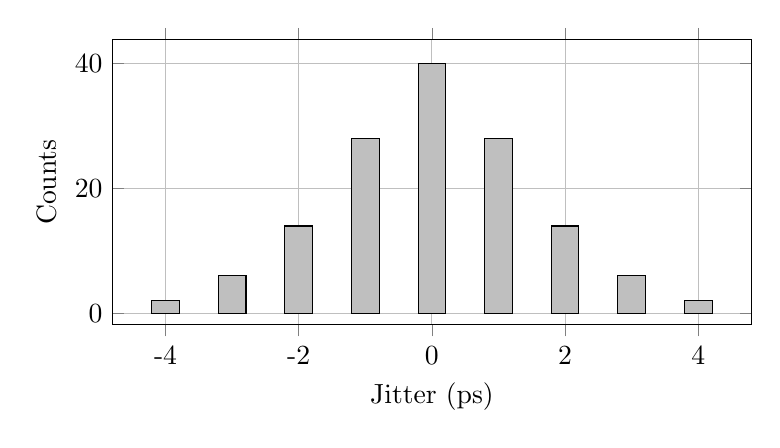
\begin{tikzpicture}
    \begin{axis}[
      ybar, width=0.8\linewidth, height=5.2cm,
      xlabel={Jitter (ps)}, ylabel={Counts}, grid=both,
      symbolic x coords={-4,-3,-2,-1,0,1,2,3,4}]
      \addplot[fill=gray!50] coordinates{(-4,2) (-3,6) (-2,14) (-1,28) (0,40) (1,28) (2,14) (3,6) (4,2)};
    \end{axis}
  \end{tikzpicture}
  \caption{Example zero-crossing jitter histogram from transient-noise simulation}
\end{figure}

\section{Experimental evaluation: Phase noise from transient (Ring VCO)}
For the Ring VCO, when Pnoise is not available, we extract phase from the transient waveform and estimate \(\mathcal{L}(f)\) using Welch, as described earlier. The figure below is generated automatically by the notebook.

\begin{figure}[H]
  \centering
  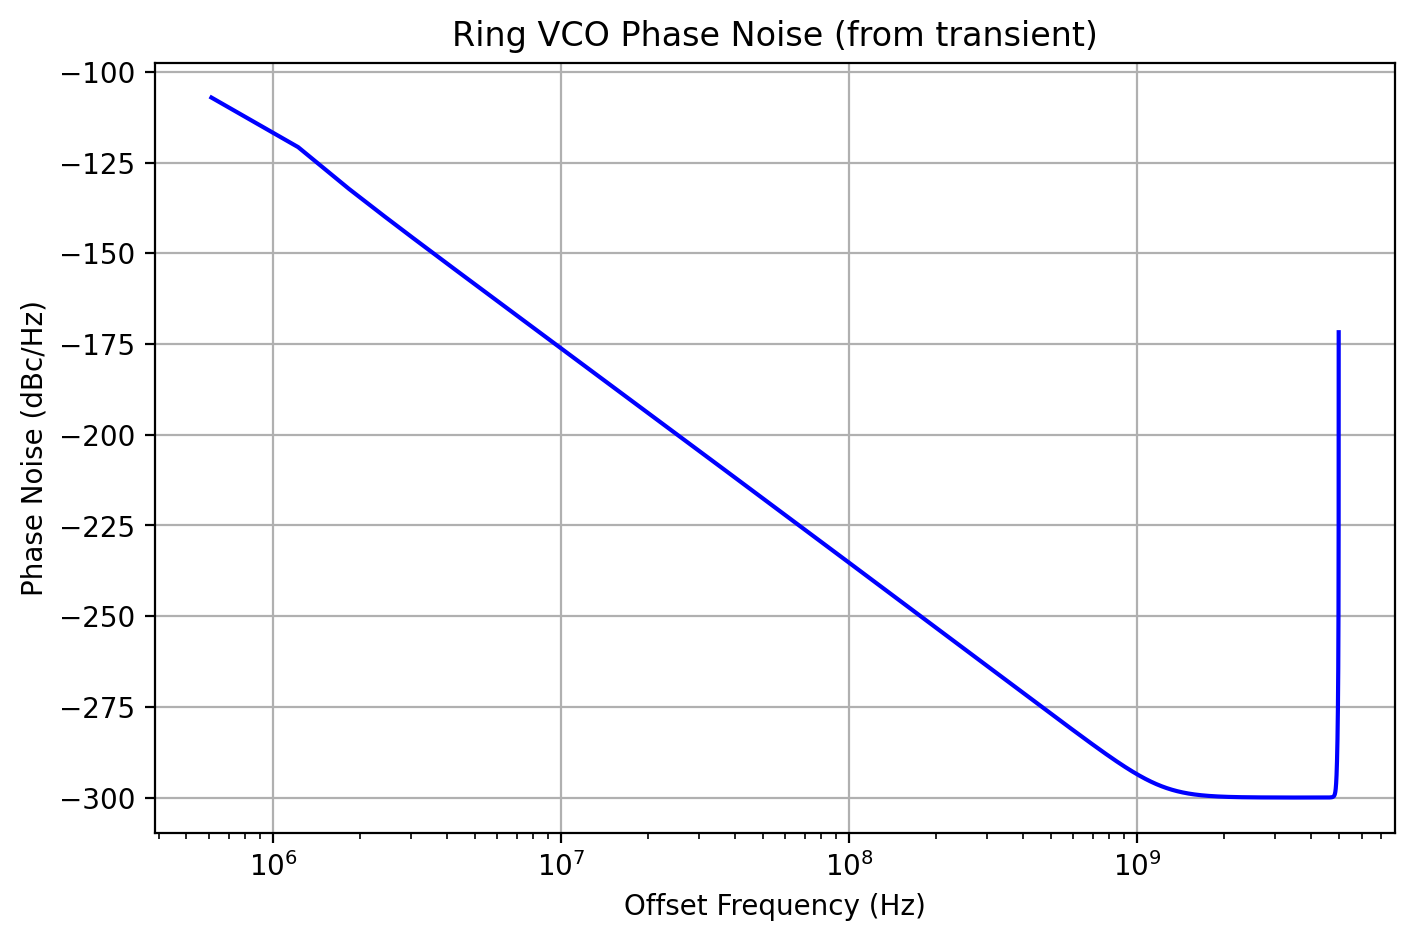
\includegraphics[width=0.9\linewidth]{ring_vco_pn_transient.png}
  \caption{Phase noise ước lượng từ transient cho Ring VCO}
\end{figure}



